\section{Le prototype : architecture et choix techniques}
Le prototype interne, développé sous le framework open source Python-Django par le responsable du \ac{DIT} de la Bibliothèque Cujas, s'inscrit dans une rupture avec le système historique \ac{XTF}. Ce dernier, bien que bénéficiant d'une solide réputation dans le monde anglo-saxon, est devenu aujourd'hui obsolète du à l'absence de mise à jour depuis 2018. Cette situation engendre d'importants risque de sécurité, une menace de rupture de service par le réseau Renater et une déconnexion par rapport aux standards utilisées. Ce sont ces multiples raisons qui ont poussé le responsable à développer ce prototype. Ce prototype a été réfléchi et conçu afin de sortir la bibliothèque de son isolement fonctionnel.

\subsection{Le dépassement de l'arborescence \enquote{à plat} et la modélisation hiérarchique}
L'un des obstacles majeurs identifiés lors de l'audit de la première bibliothèque numérique, CujasNum réside dans la rigidité architecturelle développé sous \ac{XTF}. Cette infrastructure limitait l'implémentation d'autres types de documents nécessitant une arborescence complexe. En effet, comme le souligne Isabelle Westeel, \enquote{toute gestion de collections numériques impose de tenir compte de la granularité (physique ou logique)} \footcite{westeelIndexerStructurerEchanger2010}. La structure \enquote{à plat} du logiciel a donc imposé à la Bibliothèque Cujas la diffusion de monographies uniquement sur CujasNum. 

Pour le \ac{DPRE}, cette contrainte technique empêchait l'intégration de revues juridiques. Un périodique est par nature ce que l'on qualifie \enquote{d'un objet composé (compound object)}, c'est-à-dire un \enquote{assemblage de texte}, dont l'arborescence doit être préservée pour ne pas en perdre l'intelligibilité scientifique. Une revue est composé différemment d'une monographie. Elle se compose alors \enquote{d'un titre, de l'année de publication, du volume} au minimum, mais aujourd'hui le \ac{DPRE} requiert une granularité jusqu'à l'article lui-même \footannexe{\nameref{annexe_A_rapport_audit}.}. 

Pour surmonter ces contraintes structurelles et logicielles, la transition de CujasNum vers la future plateforme ne peut se concevoir comme une simple mise à niveau technique menée en vase clos. Elle requiert un profond changement de paradigme méthodologique, passant d'une approche centrée sur le produit à une démarche centrée sur l'utilisateur. Comme le met en lumière Elina Leblanc dans ses travaux, la définition d'une offre de services pertinente exige de s'appuyer sur une approche ascendante pour adapter l'interface aux besoins et aux pratiques réels des usagers, plutôt que d'exiger d'eux une adaptation passive à la ressource. Cette primauté de l'expérience d'usage trouve son assise théorique dans le modèle de Jesse James Garrett, pour qui l'expérience utilisateur doit constituer l'élément central de la conception de tout site web \footcite{leblancBibliothequesNumeriquesEnrichies}. 

La souplesse du prototype permet selon le responsable du \ac{DIT} \enquote{d'introduire une modélisation de données à plusieurs niveaux}, et permet ainsi d'ajouter d'autres formats de documents sans avoir à \enquote{créer artificiellement des tables des matières pour pouvoir les intégrer}. Sous \ac{XTF}, la notion de \enquote{collections} était absente : toute création de collection était impossible. Celle créée sur CujasNum relève \enquote{d'un bricolage maison: réalisé à l'aide d'une requête \ac{SQL}}, permettant de la constituer \footannexe{\nameref{annexe_A_rapport_audit}}. Désormais, le prototype résout cet obstacle rencontré par les experts métiers en mettant directement à leur disposition la possibilité, dans le back-office, de pouvoir créer des collections à l'aide de sets dynamiques. Le système offre la possibilité de les créer à l'aide de plusieurs filtres que l'expert métier peut lui-même constituter : par sujet ou indexation thématique, par cote ou classification Dewey, par couverture spatiale ou géographique ou par lot de numérisation ou par critère temporel. Sur le plan technique, cette agilité repose sur la transition du Dublin Core simple vers le Dublin Core qualifié, c'est-à-dire \enquote{des élements de raffinements peuvent compléter certains éléments}, remplaçant \enquote{les éléments de base par des éléments plus précis}. \enquote{Ainsi, au lieu de title (dc:title), on pourra utiliser alternative (dcterms: alternative) pour désigner un titre abrégé ou un titre traduit} \footcite{lavennedelamontoiseOAIPMHPMHLheure2020}. Cela permet aux usagers, une navigation plus fluide. Ce prototype offre la possibilité de disposer d'une navigation ergonomique et d'une indexation fine plus agréable pour les usagers de la bibliothèque numérique, ainsi qu'une promesse de confort pour les experts métiers dans le back-office.

Au delà, du confort que cela apporte sur la page d'accueil de la bibliothèque numérique, l'implémentation de ces sets revêt un intérêt stratégique majeur pour l'interopérabilité de la \ac{BIU Cujas}. En effet, l'activation d'un entrepôt \ac{OAI-PMH} permet au prototype d'exposer ces sets de manière structurée, favorisant un moissonnage sélectif par les autres institutions patrimoniales, comme la \ac{BNF}. Comme le souligne Vincent de Lavenne, le moissonnage sélectif permet \enquote{aux fournisseurs de service de sélectionner les données qu'ils moissonnent, et donc de proposer un service pertinent}, évitant le stockage inutile de l'information et \enquote{de construire un accès adapté aux archives ouvertes} \footcite{lavennedelamontoiseOAIPMHPMHLheure2020}. 

\subsection{La déconnexion du traitement des images par le standard IIIF}
Sous CujasNum, pour consulter des ouvrage volumineux, les usagers n'avaient d'autres choix que de télécharger des fichiers \ac{PDF} extrêmement lourds, pouvant atteindre \enquote{des tailles de 300 à 400 go}. Une telle concentration de données provoquait des saturations systématiques de la bande passante et \enquote{des échecs de téléchargements récurrents}, générant une frustration chez les chercheurs et un abandon des étudiants face à ces \ac{PDF} massifs. 

Pour surmonter cette limite de performance, le prototype opère une transition architecturale en séparant la gestion des données de celle des images. Il s'appuie sur le serveur \ac{IIIF} indépendant. Ce protocole, devenu le standard incontournable des grandes institutions patrimoniales françaises et internationales, fonctionne de manière découplée : entre la distribution des images à la demande et la génération de manifestes \ac{JSON}. Ce manifeste est produit automatiquement sous le format \ac{JSON-LD}. Ce fichier de métadonnées, extrêmement léger, décrit la structure intellectuelle du document avec l'ordre des pages et l'emplacement physique des images, permettant ainsi aux chercheurs d'exploiter les données brutes et pouvant procéder à des extractions d'informations à l'aide de script.

Grâce au serveur \ac{IIIF}, le prototype propose l'intégration de deux visionneuses : la visionneuse Turner et celle plus avancée Mirador. Ce choix, peu commun, offrirait à la Bibliothèque Cujas la possibilité de concevoir une interface de consultation flexible et adaptée à différents profils d'utilisateurs : entre le grand public et le chercheur \footannexe{\nameref{annexe_A_rapport_audit}.}. Lors du benchmark réalisé autour de la réflexion menée par les bibliothèques sur la consultation de leurs documents, il apparaît que ce mode de fonctionnement a été observé uniquement dans le monde anglo-saxon, sur la Digital Bodleian Library d'Oxford et sur celle de Cambridge \footannexe{\ref{annexe_B_preconisations}.}. 

\begin{figure}[htbp]
	\centering
	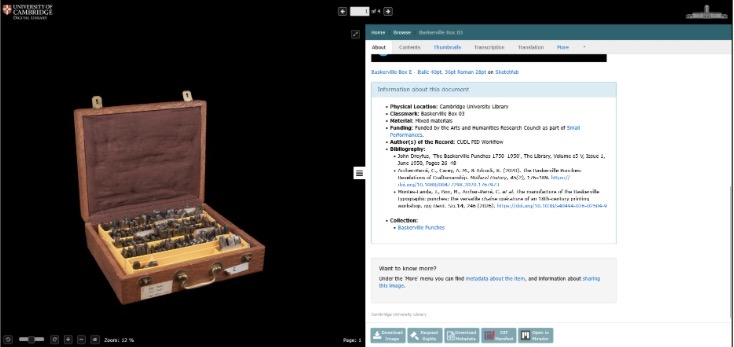
\includegraphics[width=0.8\textwidth]{./images/consultation_documents/IMG_5987.jpeg} 
	\caption{Mode de consultation proposant deux visionneuses}
	\label{fig:capture_ecran_deux_visionneuses}
\end{figure}

Une attention doit porter par la Bibliothèque Cujas face à ce choix, peu courant, car pensant s'adapter au mieux aux attentes des usagers, il ne faudrait pas que cela les rendent confus face à la présence de deux visionneuses. En effet, il semble que cela ne soit pas une habitude perpétrée par les institutions patrimoniales françaises car celle-ci propose uniquement une visionneuse \ac{IIIF}. Certains ont choisi la visionneuse Universal Viewer tandis que d'autres utilisent Mirador, répondant ainsi à des objectifs différents et des attentes propres à leurs usagers.

\subsection{L'interopérabilité des données et la pérennité des identifiants (ARK)}
Pour s'intégrer au web sémantique et aux grands réservoirs nationaux, comme le projet Orion de l'\ac{ABES}, le prototype s'appuie exclusivement sur des standards ouverts. La bibliothèque doit proposer des services permettant l'utilisation brute de données ainsi que des services d'export s'intégrant naturellement dans les chaînes de travail personnelles des chercheurs. Cette appropriation de la donnée par les chercheurs se heurte aujourd'hui à la volatilité des sessions de recherche \footannexe{\nameref{annexe_A_rapport_audit}.}.La concrétisation technique de ce "carnet de lecture" — dont nous avons justifié la nécessité méthodologique au chapitre précédent au prisme des travaux d'Elina Leblanc — pose directement la question de l'architecture de gestion des sessions dans le prototype. Afin de permettre aux chercheurs de sauvegarder leurs requêtes et leurs paniers de documents sans imposer une procédure d'inscription lourde, le prototype doit articuler deux options techniques : une persistance locale des données (via le local storage du navigateur de l'utilisateur, respectueuse de la vie privée) ou un système d'authentification fédérée (de type Shibboleth/Renater). Cette seconde piste s'avère la plus robuste pour assurer la pérennité des données de recherche d'une session à l'autre et sur différents terminaux \footcite{leblancBibliothequesNumeriquesEnrichies}. 

Afin de soutenir techniquement ces besoins d'appropriation et d'éditorialisation, l'architecture du prototype intègre des dispositifs d'interopérabilité spécifiques. Plutôt que de figer les données dans un silo de fichiers statiques, le prototype implémente des briques applicatives capables de concrétiser le concept de \enquote{citation de contenus} théorisé par Antoine Isaac, Emmanuelle Bermès et Gautier Poupeau \footcite{bermesWebSemantiqueBibliotheque2013}. En pratique, cette ambition se traduit par la mise en œuvre de modules spécifiques au sein du back-office (comme CopyIdRef ou Bibliography) et par l'exposition des métadonnées sous des formats de sérialisation ouverts (\ac{XML}, \ac{JSON-LD}). En associant à chaque document une \ac{URI} pérenne et un serveur d'images \ac{IIIF}, l'infrastructure technique ne se contente plus de diffuser : elle jette les bases d'un espace dynamique de co-construction de nouveaux savoirs, directement connectable aux outils personnels des chercheurs. Dans ce troisième âge, ce traitement intellectuel est l'un des moyens utilisés par les institutions patrimoniales transformant le document-objet en un espace d'apprentissage  et de valorisation du travail scientifique réalisés par des spécialistes.

Comme nous l'avons mis en évidence lors de l'étude comparative des outils de l'ESR, l'alternative représentée par Omeka S comporte d'importantes exigences en matière de maintenance applicative. Pour la \ac{BIU Cujas}, l'enjeu ne réside donc pas dans l'adoption passive d'un système clé en main, mais bien dans la maîtrise souveraine de ses flux de travail. En faisant le choix de développer le prototype sous Python-Django, l'institution privilégie une infrastructure sur-mesure et éco-conçue, capable de s'adapter précisément aux spécificités des sources juridiques tout en limitant la dépendance à des modules tiers dont la mise à jour n'est pas garantie à long terme.

Le choix de s'appuyer sur des formats universels et des \ac{API} vise à garantir la visibilité, la réutilisation et de la diffusion des collections à l'échelle nationale. Contrairement à l'entrepôt \ac{OAI-PMH} de CujasNum, devenu difficile à moissonner voir impossible, le prototype permet de réactiver le moissonnage en le standardisant davantage. Le système intègre dorénavant des \ac{API REST} capables de délivrer des données structurées et interopérables sous formats \ac{XML} ou \ac{JSON}, rompant avec l'image en silo \footnote{\nameref{annexe_A_rapport_audit}.}. Cette architecture modulaire offre une double opportunité : elle permet à la \ac{BIU Cujas} de moissonner d'autres portails comblant ces collections physiques ainsi que d'exposer ses propres métadonnées pour être moissonnées, augmentant drastiquement la visibilité de ses fonds.

Une des fortes attentes des chercheurs repose sur la stabilité à long terme des citations et de l'accès aux ressources numériques, pour qui la fiabilité d'un lien hypertexte est une condition importante de la scientificité de leurs travaux. À cette fin, il envisage \enquote{de désigner \ac{ARK} vers la notice bibliographique plutôt que le \ac{PDF}}. A la Bibliothèque Cujas, la méthode de création des identifiants pérennes est forgé à partir \enquote{du code-barre de l'ouvrage}, garantissant le lien permanent évitant les doublons. Cela permettrait ainsi de lier numériquement la notice bibliographique à celle du catalogue \footannexe{\nameref{annexe_A_rapport_audit}.}.

\subsection{La gestion fine des droits d'accès}
La bibliothèque numérique souhaite numériser des documents sous droit à intégrer dans sa nouvelle plateforme. Tout en restant dans un cadre strictement légal, la bibliothèque se doit de réfléchir à l'accès qu'elle permet à ses documents ne pouvant être exposés librement sans contrainte. Il est nécessaire pour l'établissement d'établir clairement une charte légale indiquant distinctement ce que l'usager a le droit de faire ou non concernant un document libre de droit et celui sous droit. La première étape consiste à assortir la notice du document à une \enquote{licence Etalab et/ou Creative Commons}. Cujas aimerait développer \enquote{un flitrage des documents sous droit ou libre de droit, grâce à la balise DcRight des notices Dublin Core} \footannexe{\nameref{annexe_A_rapport_audit}.}. 

\begin{figure}[htbp]
	\centering
	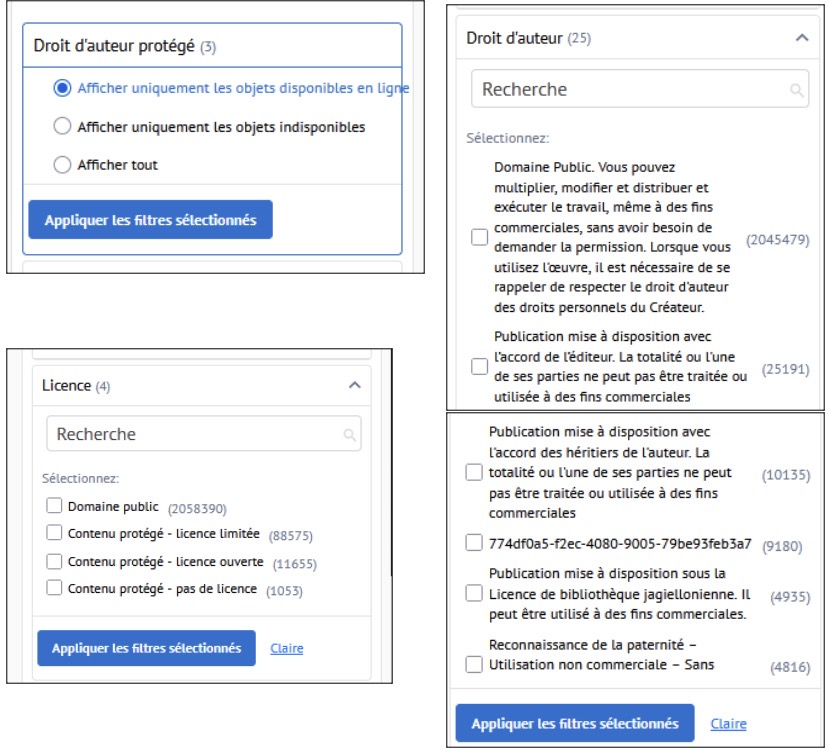
\includegraphics[width=0.5\textwidth]{./images/filtrage/IMG_5970.jpeg} 
	\caption{Différents types de filtrage dans Polona}
	\label{fig:capture_ecran_filtrage_Polona}
\end{figure}

Une des bibliothèques le fait également. Il s'agit de Polona, la bibliothèque nationale de Pologne, permettant de filtrer les documents sous droit. La deuxième étape serait de mettre en place \enquote{un horodatage débloquant le document sur le web une fois que les droits sont arrivés à terme}.

Le prototype permet de mettre en place des protocoles d'authentification centralisée \ac{SSO} et \ac{SAML}. En s'appuyant sur la fédération d'identité de Renater, grâce à ces protocoles, le système interroge à distance les serveurs des universités partenaires comme Paris I et Paris II. Cette architecture modulaire permet d'appliquer une gestion différenciée des droits d'accès \footannexe{ \nameref{annexe_A_rapport_audit}.}. Les métadonnées descriptives restent accessible publiquement sur le Web, tandis que la consultation des images est restreinte aux droits accordés par la bibliothèque en fonction du statut occupé par la personne. Un autre moyen d'accès, plus traditionnel, est de se connecter aux postes physiques connectés au réseau intranet local au sein de Cujas.

Sous \ac{XTF}, la chaîne de travail fonctionnait de façon chronophage. A l'origine, les experts métiers travaillaient de manière étanche, et toute modification de l'interface publique, une correction de coquille ou une mise en valeur éditoriale nécessitait l'intervention manuelle du service informatique. Le système était perçu comme une \enquote{boîte noire technique} par les experts métiers. Pour décloisonner ces processus, le prototype introduit un \enquote{back-office collaboratif structuré autour de profils et de rôles spécifiques}\footannexe{\nameref{annexe_A_rapport_audit} .}. 

Sur le plan de l'administration sémantique, Thomas Chaineux souligne qu'un tel environnement \enquote{répond à ses objectifs d’accès simplifié} et permet de \enquote{s’affranchir de la moindre écriture en format \ac{XML}/\ac{RDF}, \ac{JSON-LD} ou autre Turtle, grâce à l’ergonomie de son interface}. Pour la mise en valeur et l'éditorialisation, \enquote{la création de ces pages est simplifiée, de sorte qu’aucune compétence en modélisation de page Web (\ac{HTML} ou CSS) n’est requise}, l'écriture s'effectuant via une interface d'édition visuelle intuitive \footcite{chaineuxLentreeDansWeb}.

Cette autonomie s'accompagne d'une sécurisation des données grâce à la mise en œuvre de resource templates, définis par Thomas Chaineux comme \enquote{des formulaires [...] permettant de s’assurer que toutes les entités seront décrites de la même manière}, ce qui facilite la transmission et garantit la pérennité des schémas documentaires au fil du temps. Enfin, à l'image des rôles d'administration d'un \ac{CMS} sémantique, le système \enquote{propose des solutions différentes selon le statut de l’utilisateur}, permettant par exemple à un chercheur d'éditorialiser un fonds spécifique de manière autonome, tout en réservant l'accès à la base de données globale aux seuls administrateurs techniques \footcite{chaineuxLentreeDansWeb}. Cette gestion des rôles permettrait à la Bibliothèque Cujas, par exemple, \enquote{à un agent ou à un chercheur de rédiger et publier un texte sur le fonds qu'il a traité, sans pour autant lui donner les droits d'administrateur global sur tout le système}\footannexe{\nameref{annexe_A_rapport_audit}.}.    
